%%%%%%%%%%%%%%%%%%%%%%%%%%%%%%%%%%%%%%%%%%%%%%%%%%%%%%%%%%%%%%%%%%%%%%%%%%%%%%%%%%
\begin{frame}[fragile]\frametitle{}
\begin{center}
{\Large Applications}
\end{center}
\end{frame}

%%%%%%%%%%%%%%%%%%%%%%%%%%%%%%%%%%%%%%%%%%%%%%%%%%%%%%%%%%%
\begin{frame}[fragile]\frametitle{Custom Model Adaptation}
      \begin{itemize}
        \item Involves developing custom models from scratch or fine-tuning pre-existing models.
        \item Custom model development demands skilled ML scientists and substantial resources.
        \item Fine-tuning updates pre-trained models with additional data, requiring a sophisticated team.
        \item Rapid adoption across industries despite challenges and potential unintended consequences.
      \end{itemize}

\end{frame}

%%%%%%%%%%%%%%%%%%%%%%%%%%%%%%%%%%%%%%%%%%%%%%%%%%%%%%%%%%%
\begin{frame}[fragile]\frametitle{RAG-based Applications}

      \begin{itemize}
        \item Utilizes the Retrieval Augmented Generation (RAG) method.
        \item Foundational model supplemented with contextual information for efficient retrieval.
        \item Retrieves embeddings from dedicated vector databases, representing words or phrases.
        \item Bypasses traditional model limitations like context window constraints.
        \item Offers cost-effectiveness, scalability, and seamless integration into various applications and systems.
      \end{itemize}

\end{frame}

%%%%%%%%%%%%%%%%%%%%%%%%%%%%%%%%%%%%%%%%%%%%%%%%%%%%%%%%%%%
\begin{frame}[fragile]\frametitle{Generative Applications}

      \begin{itemize}
        \item Focuses on generating creative and contextually relevant content.
        \item Involves applications such as creative writing, content creation, and storytelling.
        \item Requires LLMs with strong generative capabilities and a deep understanding of context.
        \item Popular in entertainment, marketing, and industries where creative content is crucial.
      \end{itemize}
\end{frame}

%%%%%%%%%%%%%%%%%%%%%%%%%%%%%%%%%%%%%%%%%%%%%%%%%%%%%%%%%%%
\begin{frame}[fragile]\frametitle{Interactive AI Assistants}
      \begin{itemize}
        \item LLMs employed as conversational agents, providing interactive and dynamic assistance.
        \item Used in customer support, virtual assistants, and interactive chatbots.
        \item Requires real-time interaction, natural language understanding, and context-aware responses.
        \item Enhances user experience by facilitating seamless communication with AI systems.
      \end{itemize}
\end{frame}

%%%%%%%%%%%%%%%%%%%%%%%%%%%%%%%%%%%%%%%%%%%%%%%%%%%%%%%%%%%
\begin{frame}[fragile]\frametitle{Types of Tools}
  \begin{itemize}
    \item \textbf{Input Processing Tools:}
      \begin{itemize}
        \item Designed to ingest data and various inputs for the application.
      \end{itemize}
    \item \textbf{LLM Development Tools:}
      \begin{itemize}
        \item Facilitate interaction with the Large Language Model.
        \item Includes calling, fine-tuning, conducting experiments, and orchestration.
      \end{itemize}
    \item \textbf{Output Tools:}
      \begin{itemize}
        \item Utilized for managing the output from the LLM application.
        \item Focuses on post-output processes.
      \end{itemize}
    \item \textbf{Application Tools:}
      \begin{itemize}
        \item Oversee the comprehensive management of input processing, LLM development, and output tools.
        \item Includes application hosting, monitoring, and more.
      \end{itemize}
  \end{itemize}
\end{frame}


%%%%%%%%%%%%%%%%%%%%%%%%%%%%%%%%%%%%%%%%%%%%%%%%%%%%%%%%%%%
\begin{frame}[fragile]\frametitle{Tool Integration in Application Architecture}
\begin{center}
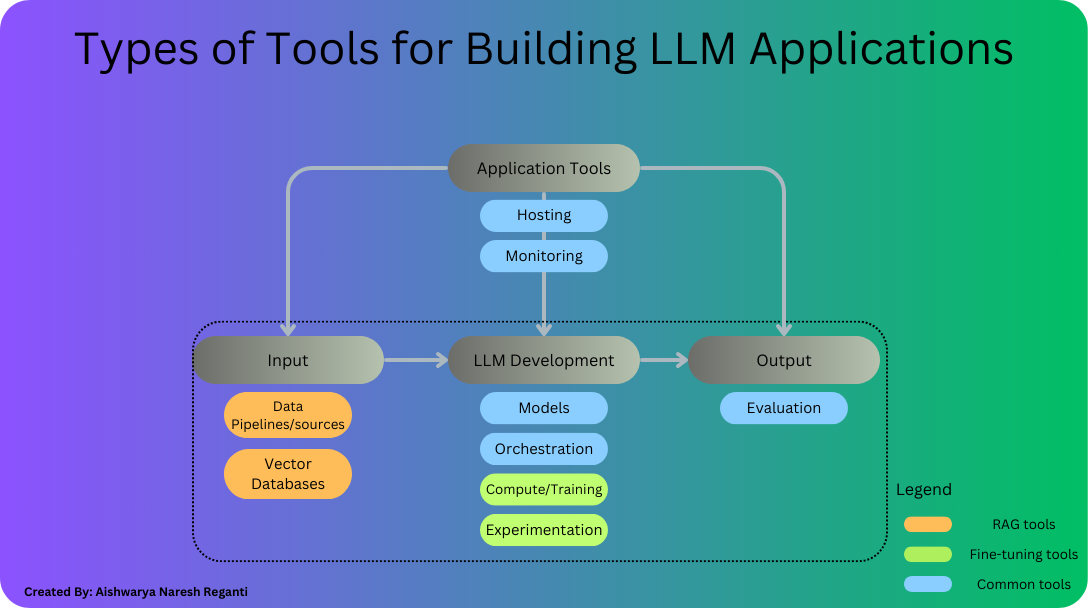
\includegraphics[width=\linewidth,keepaspectratio]{llm138}
\end{center}				

{\tiny (Ref: Applied LLMs Mastery 2024 - Aishwarya Reganti)}
\end{frame}

%%%%%%%%%%%%%%%%%%%%%%%%%%%%%%%%%%%%%%%%%%%%%%%%%%%%%%%%%%%
\begin{frame}[fragile]\frametitle{Tool Integration in Fine-Tuning Workflow}
\begin{center}
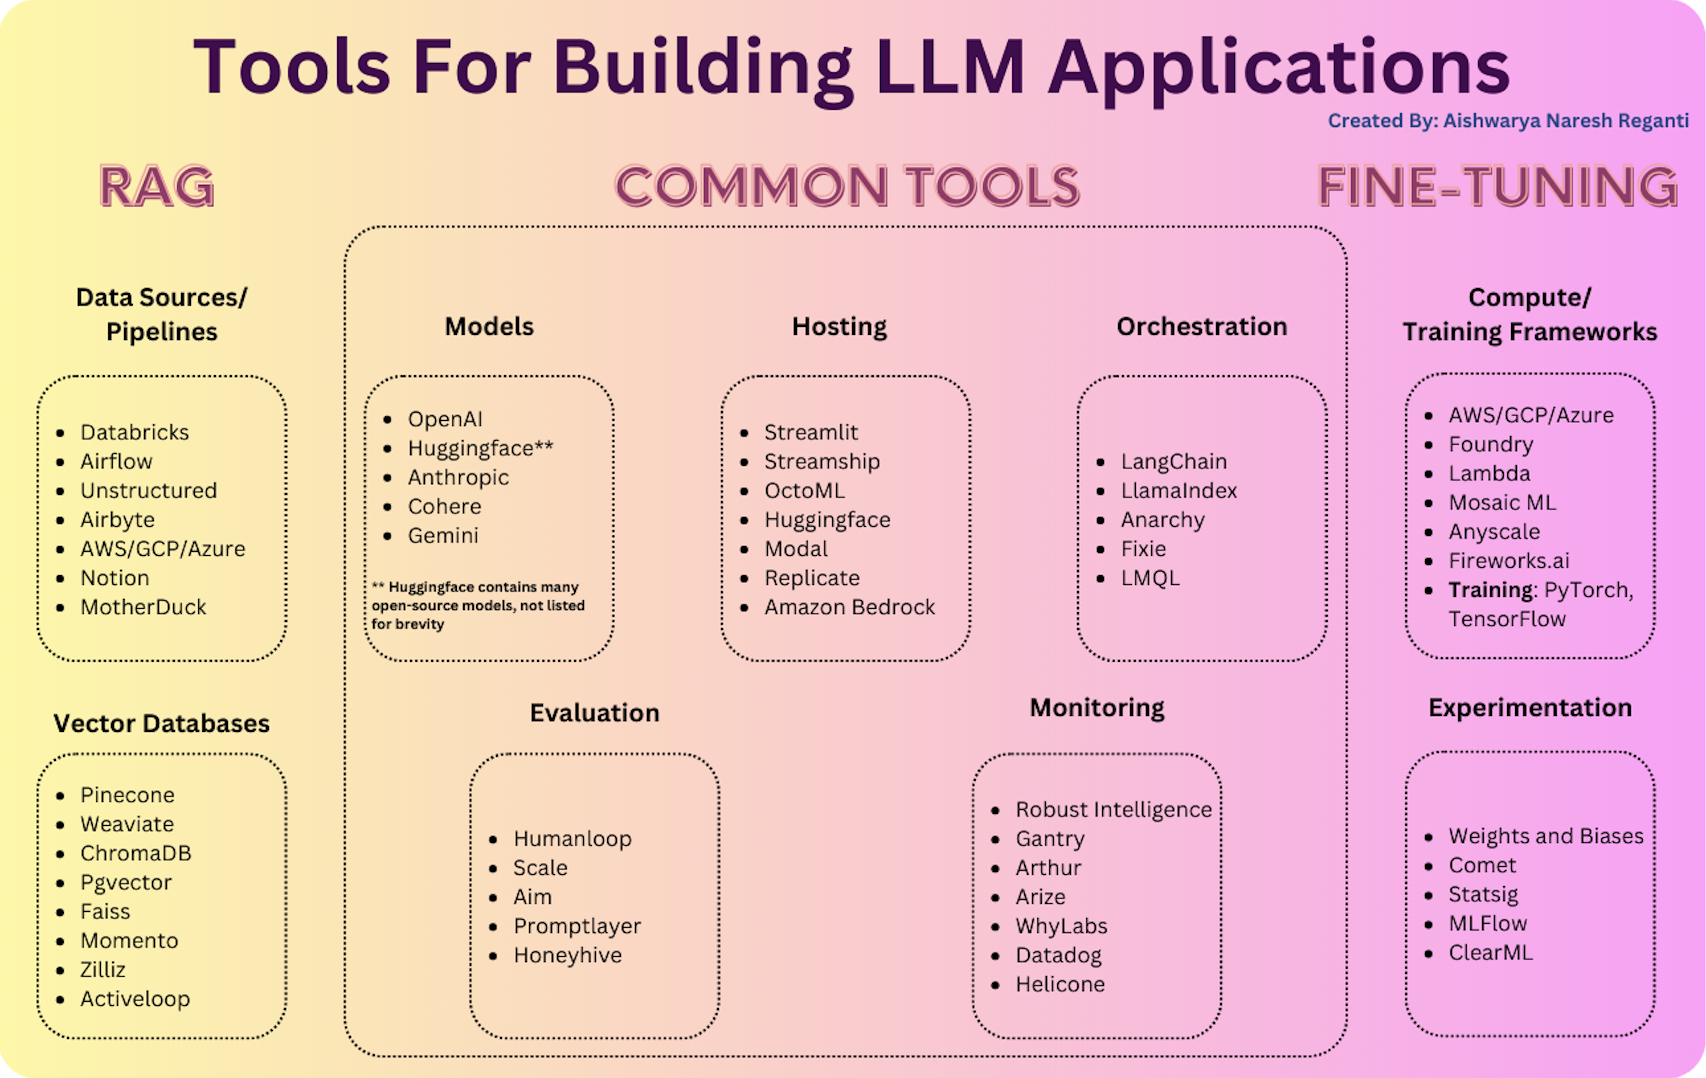
\includegraphics[width=\linewidth,keepaspectratio]{llm139}
\end{center}				

{\tiny (Ref: Applied LLMs Mastery 2024 - Aishwarya Reganti)}
\end{frame}


%%%%%%%%%%%%%%%%%%%%%%%%%%%%%%%%%%%%%%%%%%%%%%%%%%%%%%%%%%%
\begin{frame}[fragile]\frametitle{Document Question Answering Systems}

\begin{itemize}
  \item \textbf{Limited Responses:} LLMs accessing proprietary enterprise documents have responses constrained to document content.
  
  \item \textbf{Retrieval Augmentation:} A retriever identifies relevant documents, expanding LLM capabilities for more informed responses.
  
  \item \textbf{Example:} Check out the blog for a demonstration - https://lnkd.in/gJd9qfys.
\end{itemize}

\end{frame}

%%%%%%%%%%%%%%%%%%%%%%%%%%%%%%%%%%%%%%%%%%%%%%%%%%%%%%%%%%%
\begin{frame}[fragile]\frametitle{Conversational Agents}

\begin{itemize}
  \item \textbf{Customization:} LLMs customized with RAG for product manuals, domain knowledge, and guidelines.
  
  \item \textbf{Specialized Routing:} Agents can route users to more specialized agents based on queries.
  
  \item \textbf{Example:} SearchUnify's LLM+RAG conversational agent for enhanced user interaction.
\end{itemize}

\end{frame}

%%%%%%%%%%%%%%%%%%%%%%%%%%%%%%%%%%%%%%%%%%%%%%%%%%%%%%%%%%%%%%%%%%%%%%%%%%%%%%%%%%
\begin{frame}[fragile]{Real-time Event Commentary}

\begin{itemize}
  \item \textbf{Retrieval of Real-time Data:} A retriever fetches real-time updates via APIs for events like sports or news.
  
  \item \textbf{Virtual Commentator:} LLMs process the information for creating dynamic virtual commentary.
  
  \item \textbf{Example:} IBM utilized this technology for commentary during the 2023 US Open.
\end{itemize}

\end{frame}

%%%%%%%%%%%%%%%%%%%%%%%%%%%%%%%%%%%%%%%%%%%%%%%%%%%%%%%%%%%%%%%%%%%%%%%%%%%%%%%%%%
\begin{frame}[fragile]{Content Generation}

\begin{itemize}
  \item \textbf{Personalized Content:} LLMs, with RAG, personalize content for readers and incorporate real-time trends.
  
  \item \textbf{Contextual Appropriateness:} RAG ensures generated content is contextually appropriate.
  
  \item \textbf{Example:} Yarnit, an AI-based content marketing platform, employs RAG for various tasks.
\end{itemize}

\end{frame}

%%%%%%%%%%%%%%%%%%%%%%%%%%%%%%%%%%%%%%%%%%%%%%%%%%%%%%%%%%%%%%%%%%%%%%%%%%%%%%%%%%
\begin{frame}[fragile]{Personalised Recommendation}

\begin{itemize}
  \item \textbf{Evolution in Recommendations:} LLMs power the next evolution in content recommendations.
  
  \item \textbf{Game-Changer:} LLMs enhance recommendation engines in the digital economy.
  
  \item \textbf{Example:} Explore Aman Chadha's curation on LLMs in recommendation systems - https://lnkd.in/gsnnDmQS.
\end{itemize}

\end{frame}

%%%%%%%%%%%%%%%%%%%%%%%%%%%%%%%%%%%%%%%%%%%%%%%%%%%%%%%%%%%%%%%%%%%%%%%%%%%%%%%%%%
\begin{frame}[fragile]{Virtual Assistants}

\begin{itemize}
  \item \textbf{Enhancing User Experience:} Virtual personal assistants like Siri and Alexa plan to use LLMs for enhanced user experiences.
  
  \item \textbf{Personalization through Context:} With more context on user behavior, assistants become highly personalized.
\end{itemize}

\end{frame}

%%%%%%%%%%%%%%%%%%%%%%%%%%%%%%%%%%%%%%%%%%%%%%%%%%%%%%%%%%%%%%%%%%%%%%%%%%%%%%%%%%
\begin{frame}[fragile]\frametitle{AI Transforming Finance}
There are five key areas where AI can bring transformative changes to finance:
\begin{itemize}
    \item Personalize services and products
    \item Create new opportunities
    \item Manage risk and fraud
    \item Enable transparency and compliance
    \item Automate operations and reduce costs
\end{itemize}
\end{frame}

%%%%%%%%%%%%%%%%%%%%%%%%%%%%%%%%%%%%%%%%%%%%%%%%%%%%%%%%%%%%%%%%%%%%%%%%%%%%%%%%%%
\begin{frame}[fragile]\frametitle{AI in Finance: Examples}
\textbf{Personalizing Services \& Products}
\begin{itemize}
    \item Morgan Stanley: Next Best Action AI engine for tailored client messages.
    \item Klarna: Uses ChatGPT for personalized shopping suggestions.
\end{itemize}

\textbf{Creating New Opportunities}
\begin{itemize}
    \item Citadel: Negotiating enterprise-wide license for OpenAI's ChatGPT.
    \item Deutsche Bank: AI applications with NVIDIA for risk management and efficiency.
\end{itemize}

\textbf{Enabling Transparency \& Compliance}
\begin{itemize}
    \item Flagright: Introduces Flagright AI suite for global AML compliance.
\end{itemize}

\textbf{Automating Operations \& Reducing Costs}
\begin{itemize}
    \item JPMorgan: Developing IndexGPT for AI-driven financial recommendations.
\end{itemize}
\end{frame}


%%%%%%%%%%%%%%%%%%%%%%%%%%%%%%%%%%%%%%%%%%%%%%%%%%%%%%%%%%%%%%%%%%%%%%%%%%%%%%%%%%
\begin{frame}[fragile]\frametitle{Applications to Finance}
\begin{center}
\includegraphics[width=0.5\linewidth,keepaspectratio]{llm91}
\end{center}

{\tiny (Ref: LinkedIn Post - Linas Beliunas)}
\end{frame}
